    \documentclass[12pt]{article}
    \usepackage{amsfonts,amsmath,amssymb}
    \usepackage{amsmath,multicol,eso-pic}
    \usepackage[utf8]{inputenc}
    \usepackage[T1]{fontenc}
    \usepackage[left=2.00cm, right=2.00cm, top=2.00cm, bottom=2.00cm]{geometry}
    \usepackage{titlesec}
    \usepackage{enumerate}
    \usepackage{breqn}
    \usepackage{tikz}
    \usepackage{rotating}
    \usepackage{tikz}
    \usetikzlibrary{automata, positioning}
    %\renewcommand{\wedge}{~}
    %\renewcommand{\neg}{\overline}
    \titleformat{\section}{\large}{\thesection.}{1em}{}
    
    
    % % % % % POPUNITE PODATKE
    
    \newcommand{\prezimeIme}{Mašović Haris}
    \newcommand{\brIndexa}{17993}
    \newcommand{\brZadace}{3}
    
    % % % % % 
    
    \begin{document}
    
    \thispagestyle{empty}
    \begin{center}
      \vspace*{1cm}

      \vspace*{2cm}
      {\huge \bf Zadaća \brZadace } \\
      \vspace*{1cm}
      {\Large \bf iz predmeta Diskretna Matematika}

      \vspace*{1.25cm}

      {\Large Prezime i ime: \prezimeIme} \\
      \vspace*{0.5cm}
      {\Large Br. indexa: \brIndexa} \\
      \vspace*{0.5cm}
      {\Large Demonstrator: Rijad Muminović} \\
      \vspace*{0.5cm}
      {\Large Grupa: RI - 4} \\ 
      
      \vspace*{2cm}
      \renewcommand{\arraystretch}{1.75}
      \begin{tabular}{|c|c|}
    	\hline Zadatak & Bodovi \\
    	\hline 1 &  \\
    	\hline 2 &  \\
    	\hline 3 &  \\
    	\hline 4 &  \\
    	\hline 5 &  \\
    	\hline 6 &  \\
    	\hline 7 &  \\
    	\hline 8 &  \\
    	\hline 9 &  \\
    	\hline
     \end{tabular}

      \vfill


      {\large Elektrotehnički fakultet Sarajevo, Decembar 2017g.}

    \end{center}
    \newpage
    \thispagestyle{empty}
    
    
    % % % % % Rješenja zadataka
	\begin{enumerate}
		\item Rješenje zadatka \\
		\\
		Zadatak 1 [0.25 poena] \\
        \\
Neki eksperiment može dovesti do tri moguća događaja $A_1$, $A_2$ ili $A_3$ iz skupa događaja X. Ova tri događaja imaju respektivno vjerovatnoće 0.2, 0.6 i 0.2. Rezultati tog eksperimenta nisu dostupni direktno, ali se može izvesti testni eksperiment koji daje događaje $B_1$, $B_2$, $B_3$, $B_4$ ili $B_5$ iz skupa događaja Y, koji su u određenoj vezi sa događajima A1, A2 i A3. Vjerovatnoće da testni eksperiment rezultira događajem $B_j$, j = 1, 2, 3, 4, 5 ukoliko je izvorni eksperiment rezultirao događajem $A_i$, i = 1, 2, 3 date su u sljedećoj tabeli: \\

\begin{tabular}{|c|c|c|c|c|c|}
\hline
p(${B_j}$/${A_i}$) & ${B_1}$   & ${B_2}$   &  ${B_3}$  & ${B_4}$ & ${B_5}$   \\ \hline
${A_1}$                           & 0.2  & 0.35 & 0.05 & 0.1  & 0.3  \\ \hline
${A_2}$                          & 0.45 & 0.15 & 0.1  & 0.15 & 0.15 \\ \hline
${A_3}$                         & 0.45 & 0.1  & 0.3  & 0.05 & 0.1  \\ \hline
\end{tabular} \\ 
\\ 
\\ 
Odredite entropije skupa izvornih i testnih događaja H(X) i H(Y), uvjetne entropije H(X/Y) i H(Y/X), zajedničku entropiju H(X,Y) te srednju količinu informacije I(X,Y) koju testni događaji nose o izvornim događajima. \\
\\
* S obzirom da imamo vjerovatnoće događaja X možemo odmah izračunati
entropiju H(X):
\begin{equation*}
    H(X) = - \sum_{i = 1}^3 P(X_i) \cdot log_2~(P(X_i))
\end{equation*}
odnosno:
\begin{equation*}
    H(X) = - (0.2 \cdot log_2~0.2 + 0.6 \cdot log_2~0.6 + 0.2 \cdot log_2~0.2) = 1.37095
\end{equation*}
Da bi izračunali entropiju H(Y) potrebne su nam sve vjerovatnoće
P($Y_j$), j {$\in$} \{1,..,5\}. Za računanje tih vjerovantoća koristit ćemo formulu
\begin{equation*}
    P(Y_j) = \sum_{i = 1}^3 P(A_i) \cdot P(B_j/A_i) = \sum_{i = 1}^3 P(B_jA_i)
\end{equation*}
odnosno to možemo uraditi sumirajući kolone preko tabele:  \\
\\
\begin{tabular}{|c|c|c|c|c|c|}
\hline
p(${B_j}$${A_i}$) & ${B_1}$   & ${B_2}$   &  ${B_3}$  & ${B_4}$ & ${B_5}$   \\ \hline
${A_1}$                           & 0.04  & 0.07 & 0.01 & 0.02  & 0.06  \\ \hline
${A_2}$                          & 0.27 & 0.09 & 0.06  & 0.09 & 0.09 \\ \hline
${A_3}$                         & 0.09 & 0.02  & 0.06  & 0.01 & 0.02  \\ \hline
\end{tabular} \\
\\ 

Sada možemo izračunati vjerovatnoće P(${Y_j}$); j = 1..5 i to:
\begin{equation*}
    P(B_1) = 0.04 + 0.27 + 0.09 = 0.4 \quad P(B_2) = 0.07 + 0.09 + 0.02 = 0.18
\end{equation*}
\begin{equation*}
    P(B_3) = 0.01 + 0.06 + 0.06 = 0.13 \quad P(B_4) = 0.02 + 0.09 + 0.01 = 0.12
\end{equation*}
\begin{equation*}
    P(B_5) = 0.06 + 0.09 + 0.02 = 0.17
\end{equation*}
\newpage
Sada možemo izračunati H(Y):
\begin{equation*}
    H(Y) = - \sum_{i = 1}^5 P(Y_i) \cdot log_2~(P(Y_i))
\end{equation*}
odnosno:
\begin{equation*}
    H(Y) = - (0.4 \cdot log_2~0.4 + 0.18 \cdot log_2~0.18 + 0.13 \cdot log_2~0.13
    + 0.12 \cdot log_2~0.12 + 0.17 \cdot log_2~0.17)
\end{equation*}
odnosno:
\begin{equation*}
    H(Y) = 2.15838
\end{equation*}
Izračunati ćemo H(X,Y) preko gornje tabele tako da posmatramo svaki broj unutar tabele:
\begin{equation*}
    H(X,Y) = - \sum_{i = 1}^3\sum_{j = 1}^5 P(B_jA_i) \cdot log_2~(P(B_jA_i)) = 3.417059
\end{equation*}
Sad ćemo izračunati H(X/Y), H(Y/X), I(X,Y):
\begin{equation*}
    H(X/Y) = H(X,Y) - H(Y) = 3.417059 - 2.15838 = 1.258679
\end{equation*}
\begin{equation*}
    H(Y/X) = H(X,Y) - H(X) = 3.417059 - 1.37095 = 2.046109
\end{equation*}
\begin{equation*}
    I(X,Y) = H(X) - H(X/Y) = 1.37095 - 1.258679 = 0.112271
\end{equation*}
		\item Rješenje zadatka \\
		\\
		Zadatak 2 [0.25 poena] \\
        \\
Na nekom fakultetu, troškove studija za 37\% studenata plaća država, dok su ostali studenti samofinansirajući. Među studentima koji se školuju o trošku države, 54\% studenata stanuje u studentskom domu, dok među samofinansirajućim studentima 39\% studenata stanuje u studentskom domu. Svi studenti koji stanuju u studentskom domu ujedno posjeduju i iskaznicu za subvencionirani javni prevoz, dok među studentima koji ne stanuju u studentskom domu istu iskaznicu posjeduje i 44\% studenata čiji studij plaća država te 45\% samofinansirajućih studenata. \\
\\
Odredite koliku prosječnu količinu informacije saznanje o tome posjeduje li student iskaznicu za subvencionirani javni prenos ili ne nosi o načinu finansiranja njegovog studija (tj. da li ga finansira država ili troškove snosi sam). \\
\\

* Skup događaja "troškove studija studenta plaća država" i "student je samofinansirajući" možemo
označiti sa X, pri čemu će prvi događaj biti $X_1$ a drugi događaj $X_2$. Na osnovu postavke zadatka,
poznato je da za ove događaje vrijedi da je 
\begin{equation*}
    p(X_1) = 0.37 \quad p(X_2) = 0.63
\end{equation*}
\newpage

Pored ovog skupa događaja, može se formirati i skup događaja {Y1, Y2} označen sa Y, čiji elementi
respektivno označavaju događaje "student stanuje u studentskom domu" i "student ne stanuje u
studentskom domu". Zadane su uslovne vjerovatnoće
\begin{equation*}
    p(Y_1/X_1) = 0.54 \quad p(Y_1/X_2) = 0.39
\end{equation*}
		
Pošto je neophodno da vrijedi da svaki student čije troškove studija plaća država ili stanuje ili ne
stanuje u studentskom domu, te analogno za studente koji su samofinansirajući, vrijede sljedeće relacije:
\begin{equation*}
    p(Y_1/X_1) + p(Y_2/X_1) = 1 \quad p(Y_1/X_2) + p(Y_2/X_2) = 1
\end{equation*}
na osnovu čega se mogu izračunati tražene vjerovatnoće:
\begin{equation*}
    p(Y_2/X_1) = 1 - p(Y_1/X_1) = 0.46 \quad p(Y_2/X_2) = 1 - p(Y_1/X_2) = 0.61
\end{equation*}
Dalje, potrebno je uvesti i skup događaja Z sa događajima \{$Z_1$, $Z_2$\} koji respektivno predstavljaju
tvrdnje „student posjeduje iskaznicu za subvencionirani javni prevoz“ i „student ne posjeduje
iskaznicu za subvencionirani javni prevoz“. S obzirom na činjenicu da svi studenti koji stanuju u
studentskom domu također posjeduju iskaznicu za subvencionirani javni prevoz, dolazi se do
zaključka da najmanje 54\% studenata čije troškove studija plaća država te 39\%
samofinansirajućih studenata posjeduje iskaznicu. Također, s obzirom na to da i među studentima
koji ne stanuju u domu iskaznicu ima 44\% studenata sa državnog budžeta, vjerovatnoća da
student posjeduje iskaznicu uz uslov da mu troškove studija plaća država računa se kao:		
0.54 + 0.44 ${\cdot}$ (1 - 0.54) = 0.7424. Dobijena vjerovatnoća po već uvedenim
oznakama predstavlja vjerovatnoću p($Z_1$/$X_1$).  Jasno je da svaki student čije troškove studija plaća
država ili ima ili nema iskaznicu, pa je vjerovatnoća p($Z_2$/$X_1$) = 1 - 0.7424 = 0.2576.
\\
\\
Na analogan način računa se vjerovatnoća da student posjeduje iskaznicu uz uslov da je samofinansirajući, te ona iznosi 0.39 + 0.45 ${\cdot}$ (1 - 0.39) = 0.6645. Ovo je naša uvjetna vjerovatnoća p($Z_1$/$X_2$), odnosno njena suprotna vjerovatnoća je p($Z_2$/$X_2$) = 1 - 0.6645 = 0.3355. Za četiri dobijene vrijednosti najpreglednije je formirati tabelu: \\
\\
\begin{tabular}{|c|c|c|c|c|c|}
\hline
p(${Z_j}$/${X_i}$) & ${Z_1}$   &  ${Z_2}$ \\ \hline
${X_1}$                           & 0.7424  & 0.2576 \\ \hline
${X_2}$                          & 0.6645 & 0.3355 \\ \hline
\end{tabular} \\

Prosječna količina informacija koju informacija da li student posjeduje iskaznicu za
subvencionirani javni prevoz ili ne nosi o načinu finansiranja njegovog studija označava se sa
I(X, Z) i može se računati uz pomoć formule:
\begin{equation*}
    I(X,Z) = H(X) + H(Z) - H(X,Z)
\end{equation*}
Izračunajmo H(X) kao:
\begin{equation*}
    H(X) = - (p(X_1) \cdot log_2~p(X_1) + p(X_2) \cdot log_2~p(X_2)) = -(0.37 \cdot log_2~0.37 + 0.63 \cdot log_2~0.63) = 0.950672
\end{equation*}
\newpage
Izračunajmo H(Z) sada:
\begin{equation*}
    H(Z) = - (p(Z_1) \cdot log_2~p(Z_1) + p(Z_2) \cdot log_2~p(Z_2))
\end{equation*}
Vjerovatnoće p($Z_1$) i p($Z_2$) nisu poznate, ali mogu se naći i to:
\begin{equation*}
    p(Z_1) = p(X_1) \cdot p(Z_1/X_1) + p(X_2) \cdot p(Z_1/X_2) = 0.37 \cdot 0.7424 + 0.63 \cdot 0.6645 = 0.693323
\end{equation*}
\begin{equation*}
    p(Z_2) = p(X_1) \cdot p(Z_2/X_1) + p(X_2) \cdot p(Z_2/X_2) = 0.37 \cdot 0.2576 + 0.63 \cdot 0.3355 = 0.306677
\end{equation*}
Entropiju H(Z) možemo sad izračunati:
\begin{equation*}
    H(Z) = - (0.693323 \cdot log_2~0.693323 + 0.306677 \cdot log_2~0.306677) = 0.889300
\end{equation*}
Izračunajmo H(X,Z):
\begin{equation*}
    H(X,Z) = - (p(X_1Z_1) \cdot log_2~p(X_1Z_1) + p(X_2Z_1) \cdot log_2~p(X_2Z_1)~+
\end{equation*}
\begin{equation*}
    p(X_1Z_2) \cdot log_2~p(X_1Z_2) + p(X_2Z_2) \cdot log_2~p(X_2Z_2))
\end{equation*}
p($X_i$ $Z_j$) smo već faktički izračunali kod p($Z_i$) samim tim možemo samo uvrstiti pa imamo: 
\begin{equation*}
    H(X,Z) = - (0.274688 \cdot log_2~0.274688 + 0.418635 \cdot log_2~0.418635~+
\end{equation*}
\begin{equation*}
    0.095312 \cdot log_2~0.095312 + 0.211365 \cdot log_2~0.211365) = 1.83510
\end{equation*}
Na kraju I(X,Z) imamo da je:
\begin{equation*}
    I(X,Z) = H(X) + H(Z) - H(X,Z) = 0.950672 + 0.889300 - 1.83510 = 0.004872
\end{equation*}
		\item Rješenje zadatka \\
		\\
		Zadatak 3 [0.35 poena] \\

Markovljev izvor informacija prvog reda emitira četiri različite poruke a, b, c i d. Ovisno od toga koja je poruka posljednja emitirana, izvor se nalazi u jednom od 4 moguća stanja Sa, Sb, Sc i Sd koja redom odgovaraju emitiranim porukama a, b, c odnosno d. Vjerovatnoće da će izvor emitirati neku od ove 4 poruke ovisno od stanja u kojem se nalazi date su u sljedećoj tablici: \\

\begin{tabular}{|c|c|c|c|c|c|}
\hline
p(${x_j}$ / ${S_i}$) & a    & b    & c    & d    \\ \hline
${S_a}$        & 0.4  & 0.4  & 0.1  & 0.1  \\ \hline
${S_b}$        & 0.35 & 0.25 & 0.25 & 0.15 \\ \hline
${S_c}$        & 0.15 & 0.3  & 0.05 & 0.5  \\ \hline
${S_d}$        & 0.45 & 0.25 & 0.1  & 0.2  \\ \hline
\end{tabular} \\
\\
\\
Odredite entropiju i redudansu ovog izvora, zatim entropiju sekvenci dužine 5 te vjerovatnoću pojave sekvence bdcaa.
\newpage
* Kako je red izvora r = 1, izvor možemo modelirati pomoću 4 stanja,
$S_a$, $S_b$, $S_c$, $S_d$ koja redom odgovaraju prethodno emitiranim porukama a, b, c, d. 
Grafički prikaz konačnog automata koji modelira ovaj izvor dat je na slici
ispod:	\\
\\
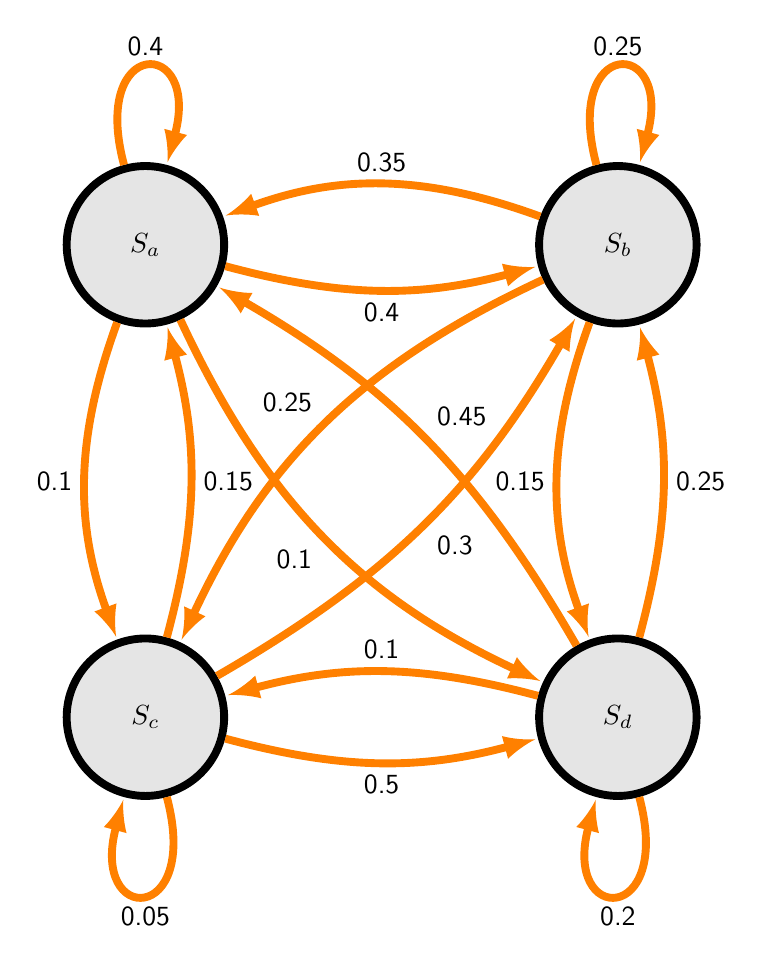
\begin{tikzpicture}[font=\sffamily]
        % Setup the style for the states
        \tikzset{node style/.style={state, 
                                    minimum width=2cm,
                                    line width=1mm,
                                    fill=gray!20!white}}
 
        % Draw the states
        \node[node style] at (0, 0)     (bull)     {${S_c}$};
        \node[node style] at (6, 0)     (bear)     {${S_d}$};
        \node[node style] at (0, 6) (stagnant) {${S_a}$};
        \node[node style] at (6, 6) (masha) {${S_b}$};
        
        % Connect the states with arrows
        \draw[every loop,
              auto=right,
              line width=1mm,
              >=latex,
              draw=orange,
              fill=orange]
            (stagnant)     edge[loop above]               node {0.4} (stagnant)
            (stagnant)     edge[bend right=15]            node {0.4} (masha)
            (stagnant)     edge[bend right=20]            node {0.1} (bull)
            (stagnant)     edge[bend right=20]            node {0.1} (bear)
            (masha)     edge[bend right=20]            node {0.35} (stagnant)
            (masha)     edge[loop above]               node {0.25} (bear)
            (masha)     edge[bend right=20]            node {0.25} (bull)
            (masha)     edge[bend right=20]            node {0.15} (bear)
            (bull)     edge[bend right=15]            node {0.15} (stagnant)
            (bull)     edge[bend right=15]            node {0.3} (masha)
            (bull)     edge[loop below]            node {0.05} (bull)
            (bull)     edge[bend right=15]            node {0.5} (bear)
            (bear)     edge[bend right=15]            node {0.45} (stagnant)
            (bear)     edge[bend right=15]            node {0.25} (masha)
            (bear)     edge[bend right=15]            node {0.1} (bull)
            (bear)     edge[loop below]            node {0.2} (bear);
\end{tikzpicture}
\\
\\
Stanje $S_a$ može nastati prelazom iz stanja $S_a$, $S_b$, $S_c$ ili $S_d$ svaki put uz
emitiranje poruke a. Na osnovu teoreme o totalnoj vjerovatnoći imamo:
\begin{equation*}
    P(S_a) = P(S_a) \cdot P(a/S_a) + P(S_b) \cdot P(a/S_b) + P(S_c) \cdot P(a/S_c) + P(S_d) \cdot P(a/S_d)
\end{equation*}
Na osnovu toga, sa svako stanje imamo: 
\begin{equation*}
    P(S_a) = 0.4 \cdot P(S_a) + 0.35 \cdot P(S_b) + 0.15 \cdot P(S_c) + 0.45 \cdot P(S_d)
\end{equation*}
\begin{equation*}
    P(S_b) = 0.4 \cdot P(S_a) + 0.25 \cdot P(S_b) + 0.3 \cdot P(S_c) + 0.25 \cdot P(S_d)
\end{equation*}
\begin{equation*}
    P(S_c) = 0.1 \cdot P(S_a) + 0.25 \cdot P(S_b) + 0.05 \cdot P(S_c) + 0.1 \cdot P(S_d)
\end{equation*}
\begin{equation*}
    P(S_a) + P(S_b) + P(S_c) = 1
\end{equation*}
Rješenja našeg sistema su respektivno:
\begin{equation*}
    P(S_a) = 0.359069 \quad P(S_b) = 0.3108426 \quad P(S_c) = 0.1396442 \quad P(S_d) = 0.1904442
\end{equation*}
\newpage
Da bi odredili entropiju izvora H(X/$X^{\infty}$) moramo odrediti entropije pojedinih stanja, odnosno H($S_a$), H($S_b$), H($S_c$), H($S_d$):
\begin{equation*}
    H(S_a) =  - (P(a/S_a) \cdot log_2~P(a/S_a) + P(b/S_a) \cdot log_2~P(b/S_a)~+
\end{equation*}
\begin{equation*}
    P(c/S_a) \cdot log_2~P(c/S_a) + P(d/S_a) \cdot log_2~P(d/S_a))
\end{equation*}
odnosno kao finalna entropija svakog stanja:
\begin{equation*}
    H(S_a) = 1.72193 \quad H(S_b) = 1.94065 \quad H(S_c) = 1.64773 \quad H(S_d) = 1.81498
\end{equation*}
Za entropiju izraza imamo:
\begin{equation*}
    H(X/X^\infty) = P(S_a)H(S_a) + P(S_b)H(S_b) + P(S_c)H(S_c) + P(S_d)H(S_d) = 1.797276726642
\end{equation*}
Redudansu izvora računamo kao:
\begin{equation*}
    R = \frac{log_2~4 - H(X/X^\infty)}{log_2~4} = \frac{2 - 1.797276726642}{2} = 0.101361636679
\end{equation*}
Vjerovatnoću sekvence ${\boldsymbol{bdcaa}}$ možemo izračunati kao
\begin{equation*}
    P(bdcaa) = P(b) \cdot P(d/b) \cdot P(c/d) \cdot P(a/c) \cdot P(a/a) = 0.3108426 \cdot 0.15 \cdot 0.1 \cdot 0.15 \cdot 0.4 = 0.00027975834
\end{equation*}
odnosno 
\begin{equation*}
    P(bdcaa) = 0.027975834\%
\end{equation*}
Za računanje entropije sekvenci dužine 5 imamo relaciju:
\begin{equation*}
    H(X^5) = H(X^1) + 4 \cdot H(X/X^\infty) 
\end{equation*}
Treba nam još entropija H($X^1$), koja iznosi:
\begin{equation*}
    H(X^1) = -(P(a) \cdot log_2~P(a) + P(b) \cdot log_2~P(b) + P(c) \cdot log_2~P(c) + P(d) \cdot log_2~P(d)) = 1.90685
\end{equation*}
Izračunajmo sada entropiju sekvenci 5:
\begin{equation*}
    H(X^5) = H(X^1) + 4 \cdot H(X/X^\infty)  = 1.90685 + 4 \cdot 1.797276726642 = 9.095956906568
\end{equation*}
		\item Rješenje zadatka \\
		\\
Zadatak 4 [0.4 poena] \\
\\
Markovljev izvor informacija drugog reda emitira dvije različite poruke 0 i 1. Ovisno od toga koje su dvije poruke posljednje emitirane, izvor se može naći u jednom od 4 moguća stanja $S_{00}$, $S_{01}$, $S_{10}$ odnosno $S_{11}$ (recimo, ukoliko su posljednje dvije emitirane poruke 0 i 1 tim redom, izvor će se nalaziti u stanju $S_{01}$). Vjerovatnoće emitiranja poruke 0 u svakom od tih stanja iznose: \\
\\
\begin{equation*}
    p(0/S_{00}) = 0.7 \quad p(0/S_{01}) = 0.6 \quad p(0/S_{10}) = 0.1 \quad p(0/S_{11}) = 0.1 
\end{equation*}
\\
Odredite entropiju i redudansu ovog izvora, zatim entropiju sekvenci dužine 6 te vjerovatnoću pojave sekvence 00110.
		\newpage
		* Kako je red izvora r = 2, izvor možemo modelirati pomoću 4 stanja $S_{00}$,
$S_{01}$, $S_{10}$ odnosno $S_{11}$. Grafički prikaz konačnog automata koji modelira ovaj
izvor prikazan je na slici ispod: \\
\\
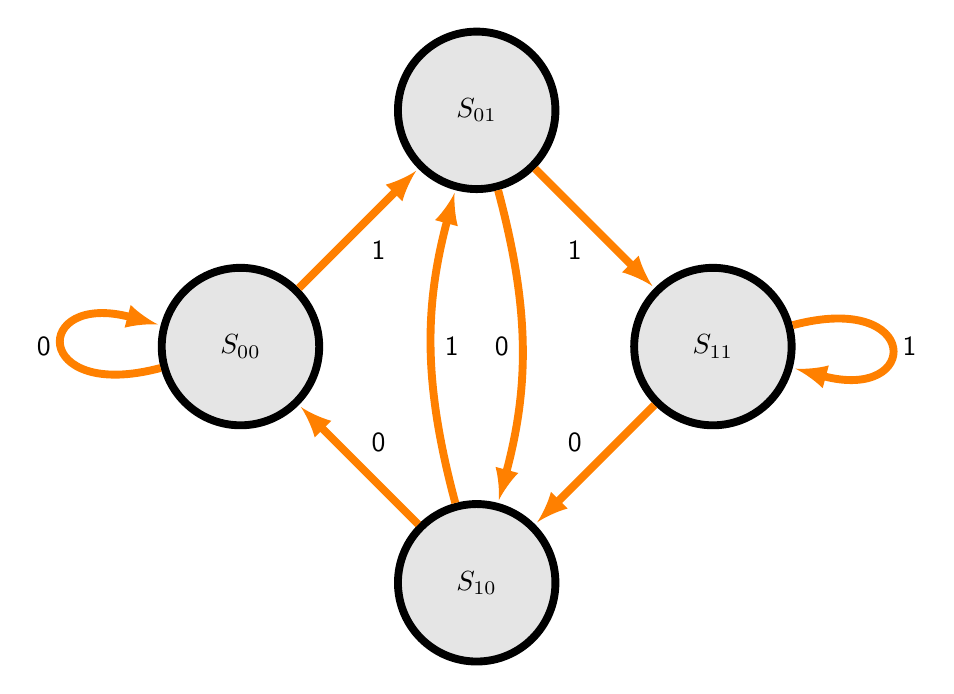
\begin{tikzpicture}[font=\sffamily]
        % Setup the style for the states
        \tikzset{node style/.style={state, 
                                    minimum width=2cm,
                                    line width=1mm,
                                    fill=gray!20!white}}
 
        % Draw the states
        \node[node style] at (0, 3)     (bull)     {${S_{00}}$};
        \node[node style] at (3, 0)     (bear)     {${S_{10}}$};
        \node[node style] at (3, 6) (stagnant) {${S_{01}}$};
        \node[node style] at (6, 3) (masha) {${S_{11}}$};
        
        % Connect the states with arrows
        \draw[every loop,
              auto=right,
              line width=1mm,
              >=latex,
              draw=orange,
              fill=orange]
            (stagnant)     edge[bend right=0]            node {1} (masha)
            (stagnant)     edge[bend left=15]            node {0} (bear)
            (bull)     edge[loop left]            node {0} (bull)
            (bull)     edge[bend left=0]            node {1} (stagnant)
            (masha)     edge[loop right]            node {1} (masha)
            (masha)     edge[bend left=0]            node {0} (bear)
            (bear)     edge[bend left=15]            node {1} (stagnant)
            (bear)     edge[bend right=0]            node {0} (bull);
\end{tikzpicture}
\\
Kako imamo vjerovatnoće emitiranja poruke 0 u svim stanjima, na osnovu
njih možemo dobiti vjerovatnoće emitiranja poruke 1 u tim istim stanjima:
\begin{equation*}
    p(1/S_{00}) = 0.3 \quad p(1/S_{01}) = 0.4 \quad p(1/S_{10}) = 0.9 \quad p(1/S_{11}) = 0.9 
\end{equation*}
Izračunajmo entropiju stanja: \\
\begin{equation*}
    H(S_{00}) = -(0.7 \cdot log_2~0.7 + 0.3 \cdot log_2~0.3) = 0.881291
\end{equation*}
\begin{equation*}
    H(S_{01}) = -(0.6 \cdot log_2~0.6 + 0.4 \cdot log_2~0.4) = 0.970951
\end{equation*}
\begin{equation*}
    H(S_{10}) = -(0.1 \cdot log_2~0.1 + 0.9 \cdot log_2~0.9) = 0.468996
\end{equation*}
\begin{equation*}
    H(S_{11}) = -(0.1 \cdot log_2~0.1 + 0.9 \cdot log_2~0.9) = 0.468996
\end{equation*}
Sada možemo postaviti sistem jednačina pomoću kojeg dobijamo vjerovatnoće svakog od stanja:
\begin{equation*}
    P(S_{00}) = 0.7 \cdot P(S_{00}) + 0.1 \cdot P(S_{10})
\end{equation*}
\begin{equation*}
    P(S_{01}) = 0.3 \cdot P(S_{00}) + 0.9 \cdot P(S_{10})
\end{equation*}
\begin{equation*}
    P(S_{11}) = 0.4 \cdot P(S_{01}) + 0.9 \cdot P(S_{11})
\end{equation*}
\begin{equation*}
    P(S_{00}) + P(S_{01}) + P(S_{10}) + P(S_{11}) = 1
\end{equation*}
Respektivno, rješenja su:
\begin{equation*}
    P(S_{00}) = 0.05263158 \quad P(S_{01}) = 0.1578947 \quad P(S_{10}) = 0.1578947 \quad P(S_{11}) = 0.6315789
\end{equation*}
Izračunajmo sada entropiju izvora
\begin{equation*}
    H(X/X^\infty) = P(S_{00})H(S_{00}) + P(S_{01})H(S_{01}) + P(S_{10})H(S_{10}) + P(S_{11})H(S_{11}) = 0.56995171513508
\end{equation*} 
\newpage
Redudansa izvora je:
\begin{equation*}
    R =  \frac{log_2~2 - 0.56995171513508}{1} = 0.43004828486492
\end{equation*}
Odredimo entropiju sekvenci dužine 6:
\begin{equation*}
    H(X^6) = H(X^2) + 4 \cdot H(X/X^\infty) 
\end{equation*}
Odredimo $H(X^2)$:
\begin{equation*}
    H(X^2) = -(P(S_{00}) \cdot log_2~P(S_{00}) + P(S_{01}) \cdot log_2~P(S_{01}) +
    P(S_{10}) \cdot log_2~P(S_{10}) + P(S_{11}) \cdot log_2~P(S_{11}))
\end{equation*}
odnosno
\begin{equation*}
    H(X^2) = 1.483226
\end{equation*}
odnosno entropija sekvenci 6 je:
\begin{equation*}
    H(X^6) = H(X^2) + 4 \cdot H(X/X^\infty) = 1.483226 + 4 \cdot 0.56995171513508 = 3.76303286054032
\end{equation*}
Izračunajmo još i vjerovatnoću sekvence 00110:
\begin{equation*}
    p(00110) = p(00) \cdot p(1/00) \cdot p(1/01) \cdot p(0/11) = 0.05263158 \cdot 0.3 \cdot 0.4 \cdot 0.1 = 0.00063157896
\end{equation*}
odnosno 
\begin{equation*}
    p(00110) = 0.063157896\%
\end{equation*}
		\item Rješenje zadatka \\
		\\
		Zadatak 5 [0.6 poena] \\
        \\
Ergodični izvor informacija bez memorije emitira 10 poruka A, B, C, D, E, F, G, H, I i J. Proučavanjem sekvence dužine 521 koju je emitirao ovaj izvor, uočena je sljedeća učestalost pojavljivanja pojedinih poruka: \\
\\
\begin{tabular}{|c|c|c|c|c|c|c|c|c|c|c|}
\hline
Poruka:     & A  & B  & C  & D  & E  & F  & G  & H  & I  & J  \\ \hline
Učestalost: & 46 & 40 & 62 & 79 & 40 & 30 & 69 & 31 & 29 & 95 \\ \hline
\end{tabular}
\\
\\
Za ovaj izvor informacija formirajte: \\
\\
a. Binarni Shannon-Fano kod sa simbolima 0 i 1; \\
b. Binarni Huffmanov kod sa simbolima 0 i 1; \\
c. Ternarni Huffmanov kod sa simbolima 0, 1 i 2. \\

Za sva tri načina kodiranja, izračunajte protok informacija kroz komunikacioni kanal, procenat iskorištenja kanala veze, te kodirajte sekvencu poruka DIHFAAHE.
		\newpage
		* a)~Konstrukcija Shannon-Fano koda prikazana je u sljedećoj tabeli, pri
čemu su u tabeli umjesto vjerovatnoća prikazane učestalosti, što se
zapravo svodi na isto, jer su učestalosti proporcionalne vjerovatnoćama. \\
\\
\begin{tabular}{|l|l|l|llllllll}
\cline{1-3}
95 J &       & \textbf{95/00} &                                      &                                       &  &  &  &  &  &  \\ \cline{1-1} \cline{3-4}
79 D & 243/0 & 148/01         & \multicolumn{1}{l|}{\textbf{79/010}} &                                       &  &  &  &  &  &  \\ \cline{1-1} \cline{4-4}
69 G &       &                & \multicolumn{1}{l|}{\textbf{69/011}} &                                       &  &  &  &  &  &  \\ \cline{1-4}
62 C &       &                & \multicolumn{1}{l|}{\textbf{62/100}} &                                       &  &  &  &  &  &  \\ \cline{1-1} \cline{4-5}
46 A &       & 130/10         & \multicolumn{1}{l|}{68/101}          & \multicolumn{1}{l|}{\textbf{46/1010}} &  &  &  &  &  &  \\ \cline{1-1} \cline{5-5}
40 B &       &                & \multicolumn{1}{l|}{}                & \multicolumn{1}{l|}{\textbf{40/1011}} &  &  &  &  &  &  \\ \cline{1-1} \cline{3-5}
40 E & 278/1 &                & \multicolumn{1}{l|}{71/110}          & \multicolumn{1}{l|}{\textbf{40/1100}} &  &  &  &  &  &  \\ \cline{1-1} \cline{5-5}
31 H &       & 148/11         & \multicolumn{1}{l|}{}                & \multicolumn{1}{l|}{\textbf{31/1101}} &  &  &  &  &  &  \\ \cline{1-1} \cline{4-5}
30 F &       &                & \multicolumn{1}{l|}{59/111}          & \multicolumn{1}{l|}{\textbf{30/1110}} &  &  &  &  &  &  \\ \cline{1-1} \cline{5-5}
29 I &       &                & \multicolumn{1}{l|}{}                & \multicolumn{1}{l|}{\textbf{29/1111}} &  &  &  &  &  &  \\ \cline{1-5}
\end{tabular}
\\
\\
Imamo kodirane sekvence:
\begin{equation*}
    A - 1010 \quad B - 1011 \quad C - 100 \quad D - 010 \quad E - 1100 \quad F - 1110 \quad G - 011 \quad H - 1101 \quad I - 1111 \quad J - 00
\end{equation*}
Izračunajmo H(X/${X^\infty}$) pri čemu sad moramo uzeti vjerovatnoće u obzir, \\odnosno  učestalost / 521:
		
\begin{equation*}
    H(X/X^\infty) = - \frac{1}{521}(95 \cdot log_2~\frac{95}{521} +	79 \cdot log_2~\frac{79}{521} +
    69 \cdot log_2~\frac{69}{521} + 62 \cdot log_2~\frac{62}{521} + 46 \cdot log_2~\frac{46}{521}~+
\end{equation*}
\begin{equation*}
	40 \cdot log_2~\frac{40}{521} + 40 \cdot log_2~\frac{40}{521} + 31 \cdot log_2~\frac{31}{521} +
	30 \cdot log_2~\frac{30}{521} + 29 \cdot log_2~\frac{29}{521})
\end{equation*}
odnosno:
\begin{equation*}
    H(X/X^\infty) = 3.20116706
\end{equation*}
Da bi izračunali prosječnu dužinu kodne riječi, ukoliko je $n_i$ dužina
kodne riječi pridružene i-toj poruci koristimo formulu:
\begin{equation*}
    n_{sr} = \frac{1}{N} \cdot \sum_{i = 1}^m N_i \cdot n_i
\end{equation*}
odnosno:
\begin{equation*}
    n_{sr} = \frac{1}{521}(95 \cdot 2 + 79 \cdot 3 + 69 \cdot 3 + 62 \cdot 3 + 46 \cdot 4 + 40 \cdot 4 + 40 \cdot 4 + 31 \cdot 4 + 30 \cdot 4 + 29 \cdot 4) = 3.232245
\end{equation*}
pa je protok informacija:
\begin{equation*}
    \overline{I(X)} = \frac{H(X/X^\infty)}{n_{sr} \cdot \tau} = \frac{0.99038}{\tau}
\end{equation*}
odakle slijedi da je iskorištenost kanala veze približno 99.038\% \\
\\
Kodirana poruka DIHFAAHE glasi (razmak između svakog slova): \\
010 1111 1101 1110 1010 1010 1101 1100
		\newpage
b) Binarni Huffmanov kod sa 0 i 1: \\
\\
\begin{tabular}{|l|l|l|l|l|l|l|l|l|l|}
\hline
95 J & 95 J   & 95 J   & 95 J   & C/0 121 & E/00 140 & A/00 165 & C/00 216 & A/000 & \textbf{A/0000} \\ \cline{1-4}
79 D & 79 D   & 69 D   & A/0 86 & F/10    & H/01     & B/01     & F/010    & B/001 & \textbf{B/0001} \\ \cline{1-3}
69 G & 69 G   & E/0 71 & B/1    & I/11    & G/1      & D/1      & I/011    & D/01  & \textbf{D/001}  \\ \cline{1-2} \cline{4-7}
62 C & 62 C   & H/1    & 79 D   & 95 J    & C/0 121  & E/00 140 & J/1      & E/100 & \textbf{E/0100} \\ \cline{1-5} \cline{8-8}
46 A & F/0 59 & 69 G   & E/0 71 & A/0 86  & F/10     & H/01     & A/00 165 & H/101 & \textbf{H/0101} \\ \cline{1-1} \cline{3-3}
40 B & I/1    & 62 C   & H/1    & B/1     & I/11     & G/1      & B/01     & G/11  & \textbf{G/011}  \\ \cline{1-7} \cline{9-9}
40 E & 46 A   & F/0 59 & 69 G   & 79 D    & 95 J     & C/0 121  & D/1      & C/00  & \textbf{C/100}  \\ \cline{1-2} \cline{4-6} \cline{8-8}
31 H & 40 B   & I/1    & 62 C   & E/0 71  & A/0 86   & F/10     & E/00 146 & F/010 & \textbf{F/1010} \\ \cline{1-4}
30 F & 40 E   & 46 A   & F/0 59 & H/1     & B/1      & I/11     & H/01     & I/011 & \textbf{I/1011} \\ \cline{1-3} \cline{5-7}
29 I & 31 H   & 40 B   & I/1    & 69 G    & 79 D     & 95 J     & G/1      & J/1   & \textbf{J/11}   \\ \hline
\end{tabular}
\\
\\ Po formuli koju smo koristili u dijelu zadatka pod a, dobijamo da je:
\begin{equation*}
    n_{sr} = \frac{1}{521}(4 \cdot 46 + 4 \cdot 40 + 3 \cdot 79 + 4 \cdot 40 + 4 \cdot 31 +
    3 \cdot 69 + 3 \cdot 62 + 4 \cdot 30 + 4 \cdot 29 + 2 \cdot 95) = 3.232245
\end{equation*}
pa je na osnovu toga protok informacija (pošto je $n_{sr}$ i entropija izvora ista) isti kao u prethodnom zadatku, samim tim je i iskorištenost kanala veze ista. \\
\\
Kodirana poruka DIHFAAHE glasi (razmak između svakog slova): \\
001 1011 0101 1010 0000 0000 0101 0100 \\
\\
c) Ternarni Huffmanov kod sa 0, 1 i 2 : \\
\\
\begin{tabular}{|l|l|l|l|l|l|}
\hline
95 J & 95 J   & B/0 111 & C/0 167 & J/0 243 & \textbf{J/00 521} \\ \cline{1-2}
79 D & 79 D   & E/1     & F/10    & D/1     & \textbf{D/01}     \\ \cline{1-2}
69 G & 69 G   & H/2     & I/11    & G/2     & \textbf{G/02}     \\ \cline{1-3} \cline{5-5}
62 C & 62 C   & 95 J    & A/2     & C/0 167 & \textbf{C/10}     \\ \cline{1-4}
46 A & F/0 59 & 79 D    & B/0 111 & F/10    & \textbf{F/110}    \\ \cline{1-1} \cline{3-3}
40 B & I/1    & 69 G    & E/1     & I/11    & \textbf{I/111}    \\ \cline{1-3}
40 E & 46 A   & 62 C    & H/2     & A/2     & \textbf{A/12}     \\ \cline{1-5}
31 H & 40 B   & F/0 59  & 95 J    & B/0 111 & \textbf{B/20}     \\ \cline{1-2} \cline{4-4}
30 F & 40 E   & I/1     & 79 D    & E/1     & \textbf{E/21}     \\ \cline{1-4}
29 I & 31 H   & 46 A    & 69 G    & H/2     & \textbf{H/22}     \\ \hline
\end{tabular}
\\
\\
Na isti način kao u dijelovima zadatka pod a i b dobijamo da je:
\begin{equation*}
    n_{sr} = \frac{1}{521}(2 \cdot 95 + 2 \cdot 79 + 2 \cdot 69 + 2 \cdot 62 + 3 \cdot 30 +
    3 \cdot 29 + 2 \cdot 46 + 2 \cdot 40 + 2 \cdot 40 + 2 \cdot 31) = 2.113243
\end{equation*}
Entropija nam je ista kao i pod a odnosno b, jer je isti skup podataka, pa na osnovu toga imamo protok informacija:
\begin{equation*}
    \overline{I(X)} = \frac{H(X/X^\infty)}{n_{sr} \cdot \tau} = \frac{1.5148125}{\tau}
\end{equation*}
Kako je kapacitet kanala veze $C_c$ = ${\frac{log_2 3}{\tau}}$ = ${\frac{1.5850}{\tau}}$ iskorištenost kanala veze je \\ ${\frac{1.5148125}{1.5850}}$ = 0.955717 = 95.5717\%
		\newpage
Kodirana poruka DIHFAAHE glasi (razmak između svakog slova): \\
01 111 22 110 12 12 22 21 
		\item Rješenje zadatka \\
		\\
		Zadatak 6 [0.7 poena] \\
        \\
Izvor informacija bez memorije emitira 4 poruke A, B, C i D. Vjerovatnoće pojavljivanja ovih poruka iznose:
\\
\\
p(A) = 0.15 \\
p(B) = 0.4 \\
p(C) = 0.1 \\
p(D) = 0.35 \\
\\
Za ovaj izvor informacija formirajte \\
a. Binarni Shannon-Fano kod sa simbolima 0 i 1, \\
b. Binarni Huffmanov kod sa simbolima 0 i 1, \\
c. Binarni Shannon-Fano kod sa simbolima 0 i 1, ali kodirajući parove poruka umjesto individualnih poruka, \\
d. Binarni Huffmanov kod sa simbolima 0 i 1, ali kodirajući parove poruka umjesto individualnih poruka. \\
\\
Za sva četiri načina kodiranja, izračunajte protok informacija kroz komunikacioni kanal, procenat iskorištenja kanala veze, te kodirajte sekvencu poruka DACDACBCDB. \\
\\
* a) Binarni Shannon-Fano kod sa simbolima 0 i 1: 
\\
\\
\begin{tabular}{|l|l|ll}
\cline{1-2}
B 0.4  & \textbf{0.4/0} &                                       &                                        \\ \cline{1-3}
D 0.35 &                & \multicolumn{1}{l|}{\textbf{0.35/10}} &                                        \\ \cline{1-1} \cline{3-4} 
A 0.15 & 0.6/1          & \multicolumn{1}{l|}{0.25/11}          & \multicolumn{1}{l|}{\textbf{0.15/110}} \\ \cline{1-1} \cline{4-4} 
C 0.1  &                & \multicolumn{1}{l|}{}                 & \multicolumn{1}{l|}{\textbf{0.1/111}}  \\ \hline
\end{tabular}
\\
\\
Iz tabele se vidi koja je poruka kodirana kojim kodom, izračunajmo entropiju izvora i prosječnu dužinu kodne riječi:
\begin{equation*}
    H(X/X^\infty) = -(0.4 \cdot log_2~0.4 + 0.35 \cdot log_2~0.35 + 0.15 \cdot log_2~0.15 + 0.1 \cdot log_2~ 0.1) = 1.80161
\end{equation*}
\begin{equation*}
    n_{sr} = 0.4 \cdot 1 + 0.35 \cdot 2 + 0.15 \cdot 3 + 0.1 \cdot 3 = 1.85
\end{equation*}
pa je protok kanala veze:
\begin{equation*}
    \overline{I(X)} = \frac{H(X/X^\infty)}{n_{sr} \cdot \tau} = \frac{0.9738}{\tau}
\end{equation*}
odnosno iskorištenost kanala veze je 97.38\%. \\
\\
Kodirana poruka DACDACBCDB glasi (razmak između svakog slova): \\
10 110 111 10 110 111 0 111 10 0 
		\newpage
b) Binarni Huffmanov kod sa simbolima 0 i 1:
\\
\\
\begin{tabular}{|l|l|l|l|}
\hline
0.4 B  & 0.4 B    & D/0 0.6 & \textbf{D/00~~~1} \\ \cline{1-2}
0.35 D & 0.35 D   & A/10    & \textbf{A/010}  \\ \cline{1-2}
0.15 A & A/0 0.25 & C/11    & \textbf{C/011}  \\ \cline{1-1} \cline{3-3}
0.1 C  & C/1      & 0.4 B   & \textbf{B/1}    \\ \hline
\end{tabular}	
\\
\\
Iz tabele se može vidjeti kojim su sekvencama slova kodirana. Entropija
je ista kao u dijelu zadatka pod a, a isti je slučaj i sa prosječnom
dužinom kodne rijeći $n_{sr}$ = 1.85, pa vrijede isti zaključci osim kodirane kodirane sekvence.
Odnosno protok kanala veze je:
\begin{equation*}
    \overline{I(X)} = \frac{H(X/X^\infty)}{n_{sr} \cdot \tau} = \frac{0.9738}{\tau}
\end{equation*}
odnosno iskorištenost kanala veze je 97.38\%. \\
\\
Kodirana poruka DACDACBCDB glasi (razmak između svakog slova): \\
00 010 011 00 010 011 1 011 00 1
\\
\\
c) Binarni Shannon-Fano kod sa simbolima 0 i 1 (parovi poruka): 
\\
\\
\begin{tabular}{|l|l|l|llll}
\cline{1-3}
BB 0,16   &        & \textbf{0,16/00} &                                          &                                           &                                            &                                             \\ \cline{1-1} \cline{3-4}
BD 0,14   & 0,44/0 & 0,28/01          & \multicolumn{1}{l|}{\textbf{0,14/010}}   &                                           &                                            &                                             \\ \cline{1-1} \cline{4-4}
DB 0,14   &        &                  & \multicolumn{1}{l|}{\textbf{0,14/011}}   &                                           &                                            &                                             \\ \cline{1-4}
DD 0,1225 &        & \textbf{}        & \multicolumn{1}{l|}{\textbf{0,1225/100}} &                                           &                                            &                                             \\ \cline{1-1} \cline{4-5}
AB 0,06   &        & 0,295/10         & \multicolumn{1}{l|}{}                    & \multicolumn{1}{l|}{\textbf{0,06/1010}}   &                                            &                                             \\ \cline{1-1} \cline{5-6}
BA 0,06   &        &                  & \multicolumn{1}{l|}{0,1725/101}          & \multicolumn{1}{l|}{0,1125/1011}          & \multicolumn{1}{l|}{\textbf{0,06/10110}}   &                                             \\ \cline{1-1}
AD 0,0525 &        &                  & \multicolumn{1}{l|}{}                    & \multicolumn{1}{l|}{}                     & \multicolumn{1}{l|}{\textbf{0,0525/10111}} &                                             \\ \cline{1-1} \cline{3-6}
DA 0,0525 &        &                  & \multicolumn{1}{l|}{}                    & \multicolumn{1}{l|}{\textbf{0,0525/1100}} &                                            &                                             \\ \cline{1-1} \cline{5-6}
BC 0,04   &        &                  & \multicolumn{1}{l|}{0,1325/110}          & \multicolumn{1}{l|}{0,08/1101}            & \multicolumn{1}{l|}{\textbf{0,04/11010}}   &                                             \\ \cline{1-1} \cline{6-6}
CB 0,04   & 0,56/1 &                  & \multicolumn{1}{l|}{}                    & \multicolumn{1}{l|}{}                     & \multicolumn{1}{l|}{\textbf{0,04/11011}}   &                                             \\ \cline{1-1} \cline{4-6}
CD 0,035  &        &                  & \multicolumn{1}{l|}{}                    & \multicolumn{1}{l|}{0,07/1110}            & \multicolumn{1}{l|}{\textbf{0,035/11100}}  &                                             \\ \cline{1-1} \cline{6-6}
DC 0,035  &        & 0,265/11         & \multicolumn{1}{l|}{}                    & \multicolumn{1}{l|}{}                     & \multicolumn{1}{l|}{\textbf{0,035/11101}}  &                                             \\ \cline{1-1} \cline{5-7} 
AA 0,0225 &        &                  & \multicolumn{1}{l|}{0,1325/111}          & \multicolumn{1}{l|}{}                     & \multicolumn{1}{l|}{0,0375/11110}          & \multicolumn{1}{l|}{\textbf{0,0225/111100}} \\ \cline{1-1} \cline{7-7} 
AC 0,015  &        &                  & \multicolumn{1}{l|}{}                    & \multicolumn{1}{l|}{0,0625/1111}          & \multicolumn{1}{l|}{}                      & \multicolumn{1}{l|}{\textbf{0,015/111101}}  \\ \cline{1-1} \cline{6-7} 
CA 0,015  &        &                  & \multicolumn{1}{l|}{}                    & \multicolumn{1}{l|}{}                     & \multicolumn{1}{l|}{0,025/11111}           & \multicolumn{1}{l|}{\textbf{0,015/111110}}  \\ \cline{1-1} \cline{7-7} 
CC 0,01   &        &                  & \multicolumn{1}{l|}{}                    & \multicolumn{1}{l|}{}                     & \multicolumn{1}{l|}{}                      & \multicolumn{1}{l|}{\textbf{0,01/111111}}   \\ \hline
\end{tabular}
\\
\\
Iz tabele se vidi koji su parovi poruka kodirani kojim kodom, izračunajmo
prosječnu dužinu kodne riječi:
\begin{equation*}
    n_{sr} = 0.16 \cdot 2 + 0.14 \cdot 3 + 0.14 \cdot 3 + 0.1225 \cdot 3 + 0.06 \cdot 4 +
    0.06 \cdot 5 + 0.0525 \cdot 5 + 0.0525 \cdot 4 + 0.04 \cdot 5 + 0.04 \cdot 5
\end{equation*}
\begin{equation*}
    + 0.035 \cdot 5 + 0.035 \cdot 5 + 0.0225 \cdot 6 + 0.015 \cdot 6 + 0.015 \cdot 6 + 0.01 \cdot 6 = 3.665
\end{equation*}
Entropija izvora je ovdje faktički entropija sekvenci dužine 2, s obzirom
da ne postoji zavisnost unazad. Pored toga, zbog nepostojanja zavisnosti unazad također vrijedi i H($X^2$) = 2 ${\cdot}$ H(X), tako da za protok
informacija dobijamo
\begin{equation*}
    \overline{I(X)} = \frac{2 \cdot H(X/X^\infty)}{n_{sr} \cdot \tau} = \frac{0.9831}{\tau}
\end{equation*}
odnosno iskorištenost kanala veze je 98.31\%. \\
Kodirana poruka DACDACBCDB glasi (razmak između svaka 2 slova): \\
1100 11100 111101 11010 011
\\
\\
d) Binarni Huffmanov kod sa simbolima 0 i 1 (parovi poruka):
\\
\\
\begin{tabular}{|l|l|l|l|l|l|ll}
\cline{1-6}
BB 0,16   & BB 0,16    & BB 0,16     & BB 0,16     & BB 0,16      & BB 0,16      &  &  \\ \cline{1-6}
BD 0,14   & BD 0,14    & BD 0,14     & BD 0,14     & BD 0,14      & BD 0,14      &  &  \\ \cline{1-6}
DB 0,14   & DB 0,14    & DB 0,14     & DB 0,14     & DB 0,14      & DB 0,14      &  &  \\ \cline{1-6}
DD 0,1225 & DD 0,1225  & DD 0,1225   & DD 0,1225   & DD 0,1225    & DD 0,1225    &  &  \\ \cline{1-6}
AB 0,06   & AB 0,06    & AB 0,06     & AB 0,06     & AA/00 0,0725 & BC/0 0,08    &  &  \\ \cline{1-4}
BA 0,06   & BA 0,06    & BA 0,06     & BA 0,06     & AC/01        & CB/1         &  &  \\ \cline{1-4} \cline{6-6}
AD 0,0525 & AD 0,0525  & AD 0,0525   & DC/0 0,06   & CD/1         & AA/00 0,0725 &  &  \\ \cline{1-3} \cline{5-5}
DA 0,0525 & DA 0,0525  & DA 0,0525   & CA/10       & AB 0,06      & AC/01        &  &  \\ \cline{1-3} \cline{5-5}
BC 0,04   & BC 0,04    & BC 0,04     & CC/11       & BA 0,06      & CD/1         &  &  \\ \cline{1-6}
CB 0,04   & CB 0,04    & CB 0,04     & AD 0,0525   & DC/0 0,06    & AB 0,06      &  &  \\ \cline{1-4} \cline{6-6}
CD 0,035  & CD 0,035   & AA/0 0,0375 & DA 0,0525   & CA/10        & BA 0,06      &  &  \\ \cline{1-2} \cline{4-4} \cline{6-6}
DC 0,035  & DC 0,035   & AC/1        & BC 0,04     & CC/11        & DC/0 0,06    &  &  \\ \cline{1-5}
AA 0,0225 & CA/0 0,025 & CD 0,035    & CB 0,04     & AD 0,0525    & CA/10        &  &  \\ \cline{1-1} \cline{3-5}
AC 0,015  & CC/1       & DC 0,035    & AA/0 0,0375 & DA 0,0525    & CC/11        &  &  \\ \cline{1-3} \cline{5-6}
CA 0,015  & AA 0,0225  & CA/0 0,025  & AC/1        & BC 0,04      & AD 0,0525    &  &  \\ \cline{1-2} \cline{4-6}
CC 0,01   & AC 0,015   & CC/1        & CD 0,035    & CB 0,04      & DA 0,0525    &  &  \\ \cline{1-6}
\end{tabular}
\\
\\
\\
\begin{tabular}{|l|l|l|l|l|ll}
\cline{1-5}
BB 0,16      & BB 0,16      & BB 0,16       & AD/00 0,185   & DD/0 0,2425   &  &  \\ \cline{1-3}
BD 0,14      & BD 0,14      & BD 0,14       & DA/01         & BA/10         &  &  \\ \cline{1-3}
DB 0,14      & DB 0,14      & DB 0,14       & BC/10         & DC/110        &  &  \\ \cline{1-3}
DD 0,1225    & DD 0,1225    & AA/000 0,1325 & CB/11         & CA/1110       &  &  \\ \cline{1-2} \cline{4-4}
AD/0 0,105   & BA/0 0,12    & AC/001        & BB 0,16       & CC/1111       &  &  \\ \cline{4-5}
DA/1         & DC/10        & CD/01         & BD 0,14       & AD/00 0,185   &  &  \\ \cline{1-1} \cline{4-4}
BC/0 0,08    & CA/110       & AB/1          & DB 0,14       & DA/01         &  &  \\ \cline{3-4}
CB/1         & CC/111       & DD 0,1225     & AA/000 0,1325 & BC/10         &  &  \\ \cline{1-3}
AA/00 0,0725 & AD/0 0,105   & BA/0 0,12     & AC/001        & CB/11         &  &  \\ \cline{5-5}
AC/01        & DA/1         & DC/10         & CD/01         & BB 0,16       &  &  \\ \cline{2-2} \cline{5-5}
CD/1         & BC/0 0,08    & CA/110        & AB/1          & BD 0,14       &  &  \\ \cline{1-1} \cline{4-5}
AB 0,06      & CB/1         & CC/111        & DD 0,1225     & DB 0,14       &  &  \\ \cline{1-5}
BA 0,06      & AA/00 0,0725 & AD/0 0,105    & BA/0 0,12     & AA/000 0,1325 &  &  \\ \cline{1-1}
DC/0 0,06    & AC/01        & DA/1          & DC/10         & AC/001        &  &  \\ \cline{3-3}
CA/10        & CD/1         & BC/0 0,08     & CA/110        & CD/01         &  &  \\ \cline{2-2}
CC/11        & AB 0,06      & CB/1          & CC/111        & AB/1          &  &  \\ \cline{1-5}
\end{tabular}
\\
\newpage
.
\\
\begin{tabular}{|l|l|l|l|l|}
\hline
DB/0 0,2725 & BB/0 0,3    & DD/00 0,4275 & BB/00 0,5725 & \textbf{BB/000~~~1}  \\
AA/1000     & BD/1        & BA/010       & BD/01        & \textbf{BD/001}    \\ \cline{2-2}
AC/1001     & DB/0 0,2725 & DC/0110      & DB/10        & \textbf{DB/010}    \\
CD/101      & AA/1000     & CA/01110     & AA/11000     & \textbf{AA/011000} \\
AB/11       & AC/1001     & CC/01111     & AC/11001     & \textbf{AC/011001} \\ \cline{1-1}
DD/0 0,2425 & CD/101      & AD/100       & CD/1101      & \textbf{CD/01101}  \\
BA/10       & AB/11       & DA/101       & AB/111       & \textbf{AB/0111}   \\ \cline{2-2} \cline{4-4}
DC/110      & DD/0 0,2425 & BC/110       & DD/00 0,4275 & \textbf{DD/100}    \\
CA/1110     & BA/10       & CB/111       & BA/010       & \textbf{BA/1010}   \\ \cline{3-3}
CC/1111     & DC/110      & BB/0 0,3     & DC/0110      & \textbf{DC/10110}  \\ \cline{1-1}
AD/00 0,185 & CA/1110     & BD/1         & CA/01110     & \textbf{CA/101110} \\ \cline{3-3}
DA/01       & CC/1111     & DB/0 0,2725  & CC/01111     & \textbf{CC/101111} \\ \cline{2-2}
BC/10       & AD/00 0,185 & AA/1000      & AD/100       & \textbf{AD/1100}   \\
CB/11       & DA/01       & AC/1001      & DA/101       & \textbf{DA/1101}   \\ \cline{1-1}
BB 0,16     & BC/10       & CD/101       & BC/110       & \textbf{BC/1110}   \\ \cline{1-1}
BD 0,14     & CB/11       & AB/11        & CB/111       & \textbf{CB/1111}   \\ \hline
\end{tabular}
\\
\\
Iz tabele se vidi koji su parovi poruka kodirani kojim kodom, izračunajmo
prosječnu dužinu kodne riječi:
\begin{equation*}
    n_{sr} = 3 \cdot  0.16 + 3 \cdot 0.14 + 3 \cdot 0.14 +  6 \cdot 0.0225 + 6 \cdot 0.015 +
    5 \cdot  0.035 + 4 \cdot 0.06 + 3 \cdot 0.1225 
\end{equation*}
\begin{equation*}
    + 4 \cdot 0.06 + 5 \cdot 0.035 + 6 \cdot 0.015 + 6 \cdot 0.01 + 4 \cdot 0.0525 +
    4 \cdot 0.0525 + 4 \cdot 0.04 + 4 \cdot 0.04 = 3.6325
\end{equation*}
Entropija izvora je ovdje faktički entropija sekvenci dužine 2, s obzirom
da ne postoji zavisnost unazad. Pored toga, zbog nepostojanja zavisnosti unazad 
također vrijedi i H($X^2$) = 2 ${\cdot}$ H(X), tako da za protok
informacija dobijamo
\begin{equation*}
    \overline{I(X)} = \frac{2 \cdot H(X/X^\infty)}{n_{sr} \cdot \tau} = \frac{0.99193}{\tau}
\end{equation*}
odnosno iskorištenost kanala veze je 99.193\%. \\
Kodirana poruka DACDACBCDB glasi (razmak između svaka 2 slova): \\
1101 01101 011001 1110 010
\\
		\newpage
		\item Rješenje zadatka \\
		\\
		Zadatak 7 [0.8 poena] \\
        \\
Markovljev izvor informacija prvog reda emitira tri različite poruke a, b i c. Ovisno od toga koja je poruka posljednja emitirana, izvor se nalazi u jednom od 3 moguća stanja $S_a$, $S_b$ i $S_c$ koja redom odgovaraju emitiranim porukama a, b odnosno c. Vjerovatnoće da će izvor emitirati neku od ove 3 poruke ovisno od stanja u kojem se nalazi date su u sljedećoj tablici: \\
		
\begin{tabular}{|l|l|l|l|}
\hline
p($x_j$ /$S_i$) & a   & b   & c   \\ \hline
$S_a$        & 0.1 & 0.2 & 0.7 \\ \hline
$S_b$        & 0.2 & 0.4 & 0.4 \\ \hline
$S_c$        & 0.6 & 0.1 & 0.3 \\ \hline
\end{tabular}
\\
\\
\\
Za ovaj izvor informacija formirajte binarni Shannon-Fano kod sa simbolima 0 i 1 \\
a. posmatrajući izvor kao izvor bez memorije; \\
b. posmatrajući izvor kao izvor bez memorije, ali kodirajući parove poruka umjesto individualnih poruka; \\
c. koristeći posebno kodiranje za svako stanje; \\
d. koristeći posebno kodiranje za svako stanje, ali kodirajući parove poruka umjesto individualnih poruka. \\
\\
Za sva četiri načina kodiranja, izračunajte protok informacija kroz komunikacioni kanal, procenat iskorištenja kanala veze, te kodirajte sekvencu poruka cbbcbaba. U posljednja dva slučaja, pretpostavite da izvor započinje rad u stanju $S_a$.

* Grafički prikaz konačnog automata koji modelira ovaj izvor dat je na slici
ispod: \\
\\
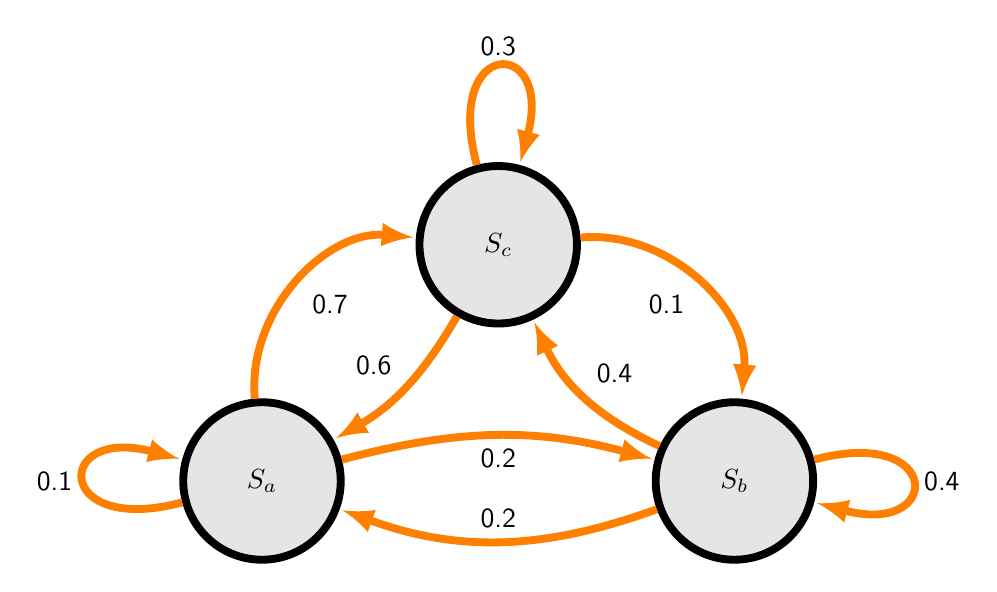
\begin{tikzpicture}[font=\sffamily]
        % Setup the style for the states
        \tikzset{node style/.style={state, 
                                    minimum width=2cm,
                                    line width=1mm,
                                    fill=gray!20!white}}
 
        % Draw the states
        \node[node style] at (0, 3)     (bull)     {${S_{a}}$};
        \node[node style] at (6, 3)     (bear)     {${S_{b}}$};
        \node[node style] at (3, 6) (stagnant) {${S_{c}}$};
        
        % Connect the states with arrows
        \draw[every loop,
              auto=right,
              line width=1mm,
              >=latex,
              draw=orange,
              fill=orange]
            (bull)     edge[loop left]            node {0.1} (bull)
            (stagnant)     edge[loop above]            node {0.3} (stagnant)
            (bear)     edge[loop right]            node {0.4} (bear)
              
            (bear)     edge[bend left=20]            node {0.4} (stagnant)    
            (bear)     edge[bend left=20]            node {0.2} (bull)   
            (bull)     edge[bend left=50]            node {0.7} (stagnant)  
            (bull)     edge[bend left=15]            node {0.2} (bear)    
            (stagnant)     edge[bend left=15]            node {0.6} (bull)  
            (stagnant)     edge[bend left=50]            node {0.1} (bear);
\end{tikzpicture}
\\
\newpage

Na osnovu teoreme o totalnoj vjerovatnoći imamo: \\
\begin{equation*}
    P(S_a) = P(S_a)P(a/S_a) + P(S_b)P(a/S_b) + P(S_c)P(a/S_c)
\end{equation*} 
\begin{equation*}
    P(S_b) = P(S_a)P(b/S_a) + P(S_b)P(b/S_b) + P(S_c)P(b/S_c)
\end{equation*} 
\begin{equation*}
    P(S_a) + P(S_b) + P(S_c) = 1
\end{equation*}
Uvrštavanjem vrijednosti iz tabele iznad dobijamo sistem jednačina čija
su rješenja:
\begin{equation*}
    P(S_a) = 0.3486239 \quad P(S_b) = 0.1926606 \quad P(S_c) = 0.4587156
\end{equation*}
Izračunajmo sada entropije svakog od stanja $S_a$, $S_b$ i $S_c$ čitajući vrijednosti
redova iz tabele i koristeći formulu za entropiju:
\begin{equation*}
    H(S_a) = 1.15678 \quad H(S_b) = 1.52193 \quad H(S_c) = 1.29546
\end{equation*}
Sada možemo izračunati entropiju izvora:
\begin{equation*}
    H(X/X^\infty) = P(S_a)H(S_a) + P(S_b)H(S_b) + P(S_c)H(S_c) = 1.290744813176
\end{equation*}
- Pređimo sada na kodiranja ($S_a$ -> a, $S_b$ -> b, $S_c$ -> c): \\
\\
a) posmatrajući izvor kao izvor bez memorije:
\\
\\
\begin{tabular}{|l|l|l}
\cline{1-2}
c 0.4587156 & \textbf{0.4587156/0} &                                            \\ \hline
a 0.3486239 & 0.5412845/1          & \multicolumn{1}{l|}{\textbf{0.3486239/10}} \\ \cline{1-1} \cline{3-3} 
b 0.1926606 &                      & \multicolumn{1}{l|}{\textbf{0.1926606/11}} \\ \hline
\end{tabular}
\\
\\
Iz tabele se vidi koji su parovi poruka kodirani kojim kodom, izračunajmo
prosječnu dužinu kodne riječi:
\begin{equation*}
    n_{sr} = 0.4587156 + 0.3486239 \cdot 2 + 0.1926606 \cdot 2 = 1.5412846
\end{equation*}
samim tim protok je: 
\begin{equation*}
    \overline{I(X)} = \frac{H(X/X^\infty)}{n_{sr} \cdot \tau} = \frac{0.837447}{\tau}
\end{equation*}
odnosno iskorištenost je: 83.74\%. \\
Kodirana poruka cbbcbaba glasi (razmak između svakog slova): \\
0 11 11 0 11 10 11 10
\\
\\
b) posmatrajući izvor kao izvor bez memorije, ali kodirajući parove poruka umjesto individualnih poruka:
\\
\\
\begin{tabular}{|l|l|l|ll}
\cline{1-3}
cc 0.21042000168 &         & \textbf{0.21042000168/00} &                                                 &                                                  \\ \cline{1-1} \cline{3-4}
ac 0.15991922146 & 0.458/0 & 0.319838442925/01         & \multicolumn{1}{l|}{\textbf{0.15991922146/010}} &                                                  \\ \cline{1-1} \cline{4-4}
ca 0.15991922146 &         &                           & \multicolumn{1}{l|}{\textbf{0.15991922146/011}} &                                                  \\ \cline{1-4}
aa 0.12153862365 &         & 0.20991504637/10          & \multicolumn{1}{l|}{\textbf{0.12153862365/100}} &                                                  \\ \cline{1-1} \cline{4-4}
bc 0.08837642272 &         &                           & \multicolumn{1}{l|}{\textbf{0.08837642272/101}} &                                                  \\ \cline{1-1} \cline{3-5} 
cb 0.08837642272 & 0.541/1 &                           & \multicolumn{1}{l|}{0.15554251246/110}          & \multicolumn{1}{l|}{\textbf{0.08837642272/1100}} \\ \cline{1-1} \cline{5-5} 
ab 0.06716608974 &         & 0.2598267090/11           & \multicolumn{1}{l|}{}                           & \multicolumn{1}{l|}{\textbf{0.06716608974/1101}} \\ \cline{1-1} \cline{4-5} 
ba 0.06716608974 &         &                           & \multicolumn{1}{l|}{0.10428419656/111}          & \multicolumn{1}{l|}{\textbf{0.06716608974/1110}} \\ \cline{1-1} \cline{5-5} 
bb 0.03711810679 &         &                           & \multicolumn{1}{l|}{}                           & \multicolumn{1}{l|}{\textbf{0.03711810679/1111}} \\ \hline
\end{tabular}
\\
\newpage
Iz tabele se vidi koji su parovi poruka kodirani kojim kodom, izračunajmo
prosječnu dužinu kodne riječi:
\begin{equation*}
    n_{sr} = 0.21042000168336 \cdot 2  +
0.15991922146284  \cdot 3 +
0.15991922146284      \cdot 3 +
0.12153862365121  \cdot 3 +
\end{equation*}
\begin{equation*}
    + 0.08837642272536     \cdot 3 + 0.08837642272536   \cdot 4 +
\end{equation*}
\begin{equation*}
0.06716608974834      \cdot 4 +
0.06716608974834      \cdot 4 +
0.03711810679236      \cdot 4 = 3.04940730733107
\end{equation*}
samim tim protok je: 
\begin{equation*}
    \overline{I(X)} = \frac{2 \cdot H(X/X^\infty)}{n_{sr} \cdot \tau} = \frac{0.846554548}{\tau}
\end{equation*}
odnosno iskorištenost je: 84.65\%. \\
Kodirana poruka cbbcbaba glasi (razmak između svaka 2 slova): \\
1100 101 1110 1110
\\
\\
c) koristeći posebno kodiranje za svako stanje:
\\
\\
$S_a$ \\
\\
\begin{tabular}{|l|l|l}
\cline{1-2}
c 0.7 & \textbf{0.7/0} &                                      \\ \hline
b 0.2 & 0.3/1          & \multicolumn{1}{l|}{\textbf{0.2/10}} \\ \cline{1-1} \cline{3-3} 
a 0.1 &                & \multicolumn{1}{l|}{\textbf{0.1/11}} \\ \hline
\end{tabular}
\\
\begin{equation*}
    n_{sr_{a}} = 0.7 + 0.4 + 0.2 = 1.3
\end{equation*}
 $S_b$ \\
\\
\begin{tabular}{|l|l|l}
\cline{1-2}
c 0.4 & \textbf{0.4/0} &                                      \\ \hline
b 0.4 & 0.6/1          & \multicolumn{1}{l|}{\textbf{0.4/10}} \\ \cline{1-1} \cline{3-3} 
a 0.2 &                & \multicolumn{1}{l|}{\textbf{0.2/11}} \\ \hline
\end{tabular}
\\
\begin{equation*}
    n_{sr_{b}} = 0.4 + 0.8 + 0.4 = 1.6
\end{equation*}
 $S_c$ \\
\\
\begin{tabular}{|l|l|l}
\cline{1-2}
a 0.6 & \textbf{0.6/0} &                                      \\ \hline
c 0.3 & 0.4/1          & \multicolumn{1}{l|}{\textbf{0.3/10}} \\ \cline{1-1} \cline{3-3} 
b 0.1 &                & \multicolumn{1}{l|}{\textbf{0.1/11}} \\ \hline
\end{tabular}
\\
\begin{equation*}
    n_{sr_{c}} = 0.6 + 0.6 + 0.2 = 1.4
\end{equation*}
 \begin{equation*}
     n_{sr} = P(S_a) \cdot n_{sr_{a}} + P(S_b) \cdot n_{sr_{b}} + P(S_c) \cdot n_{sr_{c}} = 0.3486239 \cdot 1.3 + 0.1926606 \cdot 1.6 + 0.4587156 \cdot 1.4
 \end{equation*}
 \begin{equation*}
     n_{sr} = 1.40366987
 \end{equation*} \\
  Pošto izvor započinje rad u stanju $S_a$ kodirana poruka cbbcbaba glasi (razmak po slovu):\\ 
  0 11 10 0 11 11 10 11 \\
  \\
  Protok informacija je:
 \begin{equation*}
    \overline{I(X)} = \frac{H(X/X^\infty)}{n_{sr} \cdot \tau} = \frac{0.919550}{\tau}
\end{equation*}
\\
Iskorištenost kanala veze je približno 91.955\%.
\\
\\
d) koristeći posebno kodiranje za svako stanje, ali kodirajući parove poruka umjesto individualnih poruka:
\\
$S_a$
\\	
\\
\begin{tabular}{|l|l|lllll}
\cline{1-2}
cc 0.49 & \textbf{0.49/0} &                              &                                        &                                         &                                          &                                           \\ \cline{1-4}
cb 0.14 &                 & \multicolumn{1}{l|}{0.28/10} & \multicolumn{1}{l|}{\textbf{0.14/100}} &                                         &                                          &                                           \\ \cline{1-1} \cline{4-4}
bc 0.14 &                 & \multicolumn{1}{l|}{}        & \multicolumn{1}{l|}{\textbf{0.14/101}} &                                         &                                          &                                           \\ \cline{1-1} \cline{3-5}
ac 0.07 &                 & \multicolumn{1}{l|}{}        & \multicolumn{1}{l|}{0.14/110}          & \multicolumn{1}{l|}{\textbf{0.07/1100}} &                                          &                                           \\ \cline{1-1} \cline{5-5}
ca 0.07 & 0.51/1          & \multicolumn{1}{l|}{}        & \multicolumn{1}{l|}{}                  & \multicolumn{1}{l|}{\textbf{0.07/1101}} &                                          &                                           \\ \cline{1-1} \cline{4-5}
bb 0.04 &                 & \multicolumn{1}{l|}{0.23/11} & \multicolumn{1}{l|}{}                  & \multicolumn{1}{l|}{\textbf{0.04/1110}} &                                          &                                           \\ \cline{1-1} \cline{5-6}
ab 0.02 &                 & \multicolumn{1}{l|}{}        & \multicolumn{1}{l|}{0.09/111}          & \multicolumn{1}{l|}{}                   & \multicolumn{1}{l|}{\textbf{0.02/11110}} &                                           \\ \cline{1-1} \cline{6-7} 
ba 0.02 &                 & \multicolumn{1}{l|}{}        & \multicolumn{1}{l|}{}                  & \multicolumn{1}{l|}{0.05/1111}          & \multicolumn{1}{l|}{0.03/11111}          & \multicolumn{1}{l|}{\textbf{0.02/111110}} \\ \cline{1-1} \cline{7-7} 
aa 0.01 &                 & \multicolumn{1}{l|}{}        & \multicolumn{1}{l|}{}                  & \multicolumn{1}{l|}{}                   & \multicolumn{1}{l|}{}                    & \multicolumn{1}{l|}{\textbf{0.01/111111}} \\ \hline
\end{tabular}	
\\
\\
\begin{equation*}
    n_{sr_{a}} = 0.49 + 0.14 \cdot 3 + 0.14 \cdot 3 + 0.07 \cdot 4 + 0.07 \cdot 4 + 0.04 \cdot 4 + 0.02 \cdot 5 + 0.02 \cdot 6 + 0.01 \cdot 6 = 2.33
\end{equation*}
\\
$S_b$
\\
\\
\begin{tabular}{|l|l|l|ll}
\cline{1-3}
cc 0.16 &        & \textbf{0.16/00} &                                        &                                         \\ \cline{1-1} \cline{3-4}
cb 0.16 & 0.48/0 & 0.32/01          & \multicolumn{1}{l|}{\textbf{0.16/010}} &                                         \\ \cline{1-1} \cline{4-4}
bc 0.16 &        &                  & \multicolumn{1}{l|}{\textbf{0.16/011}} &                                         \\ \cline{1-4}
bb 0.16 &        & 0.24/10          & \multicolumn{1}{l|}{\textbf{0.16/100}} &                                         \\ \cline{1-1} \cline{4-4}
ca 0.08 &        &                  & \multicolumn{1}{l|}{\textbf{0.08/101}} &                                         \\ \cline{1-1} \cline{3-5} 
ac 0.08 & 0.52/1 &                  & \multicolumn{1}{l|}{0.16/110}          & \multicolumn{1}{l|}{\textbf{0.08/1100}} \\ \cline{1-1} \cline{5-5} 
ab 0.08 &        & 0.28/11          & \multicolumn{1}{l|}{}                  & \multicolumn{1}{l|}{\textbf{0.08/1101}} \\ \cline{1-1} \cline{4-5} 
ba 0.08 &        &                  & \multicolumn{1}{l|}{0.12/111}          & \multicolumn{1}{l|}{\textbf{0.08/1110}} \\ \cline{1-1} \cline{5-5} 
aa 0.04 &        &                  & \multicolumn{1}{l|}{}                  & \multicolumn{1}{l|}{\textbf{0.04/1111}} \\ \hline
\end{tabular}
\\
\\
\begin{equation*}
    n_{sr_{b}} = 0.16 \cdot 2 + 0.16 \cdot 3 + 0.16 \cdot 3 + 0.16 \cdot 3 + 0.08 \cdot 3 + 0.08 \cdot 4 + 0.08 \cdot 4 + 0.08 \cdot 4 + 0.04 \cdot 4 = 3.12
\end{equation*}	
\\
$S_c$
\\
\\
\begin{tabular}{|l|l|l|lll}
\cline{1-3}
aa 0.36 & 0.54/0 & \textbf{0.36/00} &                                        &                                         &                                          \\ \cline{1-1} \cline{3-3}
ac 0.18 &        & \textbf{0.18/01} &                                        &                                         &                                          \\ \cline{1-4}
ca 0.18 &        & 0.27/10          & \multicolumn{1}{l|}{\textbf{0.18/100}} &                                         &                                          \\ \cline{1-1} \cline{4-4}
cc 0.09 &        &                  & \multicolumn{1}{l|}{\textbf{0.09/101}} &                                         &                                          \\ \cline{1-1} \cline{3-5}
ba 0.06 & 0.46/1 &                  & \multicolumn{1}{l|}{0.12/110}          & \multicolumn{1}{l|}{\textbf{0.06/1100}} &                                          \\ \cline{1-1} \cline{5-5}
ab 0.06 &        &                  & \multicolumn{1}{l|}{}                  & \multicolumn{1}{l|}{\textbf{0.06/1101}} &                                          \\ \cline{1-1} \cline{4-5}
cb 0.03 &        & 0.19/11          & \multicolumn{1}{l|}{}                  & \multicolumn{1}{l|}{\textbf{0.03/1110}} &                                          \\ \cline{1-1} \cline{5-6} 
bc 0.03 &        &                  & \multicolumn{1}{l|}{0.07/111}          & \multicolumn{1}{l|}{0.04/1111}          & \multicolumn{1}{l|}{\textbf{0.03/11110}} \\ \cline{1-1} \cline{6-6} 
bb 0.01 &        &                  & \multicolumn{1}{l|}{}                  & \multicolumn{1}{l|}{}                   & \multicolumn{1}{l|}{\textbf{0.01/11111}} \\ \hline
\end{tabular}
\\
\\
\begin{equation*}
    n_{sr_{c}} = 0.36 \cdot 2 + 0.18 \cdot 2 + 0.18 \cdot 3 + 0.09 \cdot 3 + 0.06 \cdot 4 + 0.06 \cdot 4 + 0.03 \cdot 4 + 0.03 \cdot 5 + 0.01 \cdot 5 = 2.69
\end{equation*}	
\newpage
Izračunajmo $n_{sr}$:
 \begin{equation*}
     n_{sr} = P(S_a) \cdot n_{sr_{a}} + P(S_b) \cdot n_{sr_{b}} + P(S_c) \cdot n_{sr_{c}} = 0.3486239 \cdot 2.33 + 0.1926606 \cdot 3.12 + 0.4587156 \cdot 2.69 
 \end{equation*}
 \begin{equation*}
     n_{sr} = 2.647339723    
 \end{equation*}
 Protok informacija je:
 \begin{equation*}
    \overline{I(X)} = \frac{2 \cdot H(X/X^\infty)}{n_{sr} \cdot \tau} = \frac{0.97512}{\tau}
\end{equation*}
\\
Iskorištenost kanala veze je približno 97.512\%. \\
\\
Pošto izvor započinje rad u stanju $S_a$ kodirana poruka cbbcbaba glasi (razmak po svakom markovljevom lancu):\\ 
100 011 1100 111110 \\
		\item Rješenje zadatka \\
		\\
		Zadatak 8 [0.25 poena] \\
        \\
Neki binarni kanal veze sa šumom prenosi dva simbola 0 i 1, pri čemu su vjerovatnoće greške nule i jedinice 0.05 i 0.2 respektivno. Odredite količinu prenesene informacije kroz ovaj kanal ukoliko vjerovatnoća pojave nule na ulazu u kanal iznosi 0.5, te odredite njegov kapacitet. \\
\\
* Ulazne simbole označimo sa $y_1$ = 0 i $y_2$ = 1, a izlazne simbole sa $z_1$ = 0 i
$z_2$ = 1. Iz postavke zadatka imamo:
\begin{equation*}
    p(z_1/y_1) = 0.95 \quad p(z_2/y_1) = 0.05 \quad p(z_1/y_2) = 0.2 \quad p(z_2/y_2) = 0.8
\end{equation*}
odnosno:
\begin{equation*}
    p(y_1) = 0.5 \quad p(y_2) = 0.5
\end{equation*}
Na osnovu teoreme o totalnoj vjerovatnoći, za vjerovatnoće simbola na
izlazu iz kanala imamo:
\begin{equation*}
    p(z_1) = p(y_1) \cdot p(z_1/y_1) + p(y2)\cdot p(z_1/y_2) =  0.5 \cdot 0.95 + 0.5 \cdot 0.2 = 0.575
\end{equation*}
\begin{equation*}
    p(z_2) = 1 - p(z_1) = 1 - 0.575 = 0.425
\end{equation*}
Za entropije ulaznih i izlaznih simbola imamo:
\begin{equation*}
    H(Y) = -(p(y_1) \cdot log_2~p(y_1) + p(y_2) \cdot log_2~p(y_2)) = 1
\end{equation*}
\begin{equation*}
    H(Z) = -(p(z_1) \cdot log_2~p(z_1) + p(z_2) \cdot log_2~p(z_2)) = 0.983708
\end{equation*}
\newpage
Za računanje uvjetne entropije H(Z/Y), koja nam treba za računanje
prenesene količine informacija, prvo ćemo odrediti "djelimično" uvjetne entropije H(Z/$y_1$) i H(Z/$y_2$):
\begin{equation*}
    H(Z/y_1) = -(p(z_1/y_1) \cdot log2(p(z_1/y_1)) + p(z_2/y_1) \cdot log2(p(z_2/y_1)) = 0.286397
\end{equation*}
\begin{equation*}
    H(Z/y_2) = -(p(z_1/y_2) \cdot log2(p(z_1/y_2)) + p(z_2/y_2) \cdot log2(p(z_2/y_2)) = 0.721928
\end{equation*}
Odavde za uvjetnu entropiju H(Z/Y) dobijamo:
\begin{equation*}
    H(Z/Y) = p(y_1) \cdot H(Z/y_1) + p(y_2) \cdot H(Z/y_2) = 0.5 \cdot 0.286397 + 0.5 \cdot  0.721928 = 0.5041625
\end{equation*}
Prenesena količina informacije kroz kanal je data sa:
\begin{equation*}
    I(Y,Z) = H(Z) - H(Z/Y) = 0.983708 - 0.5041625 = 0.4795455
\end{equation*}
    Kapacitet kanala veze je dat relacijom:
    \begin{equation*}
        C_c = \frac{1}{\tau} \cdot [~log_2~(2^{-~\frac{H_0}{\gamma}} + 2^{-~\frac{H_1}{\gamma}}) + \frac{H_0 \cdot \beta + H_1 \cdot \alpha}{\gamma}~]
    \end{equation*}
    gdje su:
    \begin{equation*}
        \alpha = 0.05 \quad \beta = 0.2 \quad H_0 = 0.286397\quad H_1 = 0.721928 \quad \gamma = 1 - \alpha - \beta = 0.75
    \end{equation*}
    Uvrštavanjem navedenih vrijednosti u formulu iznad, dobijamo da je kapacitet:
    \begin{equation*}
        C_c = \frac{0.481307}{\tau}
    \end{equation*}
		\item Rješenje zadatka \\
		\\
		Zadatak 9 [0.4 poena]
        \\
        \\
Izvor informacija bez memorije emitira dvije poruke a i b, pri čemu vjerovatnoća emitiranja poruke a iznosi p(a) = 0.3. Ove poruke se zatim kodiraju, i prenose kroz binarni kanal veze sa šumom koji koristi dva simbola 0 i 1, pri čemu su vjerovatnoće greške nule i jedinice 0.25 i 0.1 respektivno. 
\\
\\
Odredite količinu prenesene informacije kroz komunikacioni kanal, brzinu prenosa informacija kroz komunikacioni kanal, procenat iskorištenja kanala veze i vjerovatnoću greške u prenosu ukoliko se koristi: \\
\\
a. Prosto kodiranje a -> 0 i b -> 1 uz dekodiranje zasnovano na klasifikaciji $S_a$ = \{0\} i $S_b$ = \{1\}; \\
b. Zaštitno kodiranje a -> 000 i b -> 111 uz dekodiranje zasnovano na klasifikaciji $S_a$ = \{000, 001, 010, 100\} i $S_b$ = \{011, 101, 110, 111\}.
\newpage
* Ulazne simbole označimo sa $y_1$ = 0 i $y_2$ = 1, a izlazne simbole sa $z_1$ = 0 i
$z_2$ = 1. Iz postavke zadatka imamo:
\begin{equation*}
    p(z_1/y_1) = 0.75 \quad p(z_2/y_1) = 0.25 \quad p(z_1/y_2) = 0.1 \quad p(z_2/y_2) = 0.9
\end{equation*}
odnosno:
\begin{equation*}
    p(a) = 0.3 \quad p(b) = 0.7
\end{equation*}
Neka su poruke koje prima krajnji korisnik $w_1$ i $w_2$. \\
\\
a) Kako se kodiranje vrši prostim ravnomjernim kodom a -> 0 i b -> 1 (tj. a -> $y_1$ i b -> $y_2$) uz dekodiranje zasnovano na klasifkaciji $S_a$ = \{0\} i
$S_b$ = \{1\} (tj. $S_a$ = \{$z_1$\} i $S_b$ = \{$z_2$\}).\\
\\
Kako se $w_1$ dekodira samo ako je primljeno $z_1$ = 0, a $w_2$ samo ako je
primljeno $z_2$ = 1 slijedi:
\begin{equation*}
    p(w_1/a) = p(z_1/y_1) = 0.75
\end{equation*}
\begin{equation*}
    p(w_2/a) = 1 - p(w_1/a) = 0.25
\end{equation*}
\begin{equation*}
    p(w_1/b) = p(z_1/y_2) = 0.1
\end{equation*}
\begin{equation*}
    p(w_2/b) = 1 - p(w_1/b) = 0.9
\end{equation*}
Dalje imamo:
\begin{equation*}
    p(w_1) = p(a) \cdot p(w_1/a) + p(b) \cdot p(w_1/b) = 0.3 \cdot 0.75 + 0.7 \cdot  0.1 = 0.295
\end{equation*}
\begin{equation*}
    p(w_2) = 1 - p(w_1) =  0.705
\end{equation*}
Sada možemo izračunati naredno: \\
\begin{equation*}
    H(W) = -(p(w_1) \cdot log_2~p(w_1) + p(w_2) \cdot log_2~p(w_2)) = 0.875093
\end{equation*}
\begin{equation*}
    H(W/a) = -(p(w_1/a) \cdot log_2~p(w_1/a) + p(w_2/a) \cdot log_2~p(w_2/a)) = 0.811278
\end{equation*}
\begin{equation*}
    H(W/b) = -(p(w_1/b) \cdot log_2~p(w_1/b) + p(w_2/b) \cdot log_2~p(w_2/b)) = 0.468996
\end{equation*}
\begin{equation*}
    H(W/X) = p(a) \cdot H(W/a) + p(b) \cdot H(W/b) = 0.5716806
\end{equation*}
\begin{equation*}
    I(X,W) = H(W) - H(W/X) = 0.875093 - 0.5716806 = 0.3034124
\end{equation*}
Odredimo brzinu prenosa informacija kroz komunikacioni kanal:
\begin{equation*}
        \overline{I(X,W)} = \frac{I(X,W)}{\tau} = \frac{0.3034124}{\tau}
\end{equation*}
Procenat iskorištenosti kanala veze je 88.1326\% (iskorištenost u prenosu / $C_c$ - $C_c$ dobijemo po ogromnoj formuli iz 8 zadatka). Izračunajmo još
vjerovatnoću greške u prenosu: 
\begin{equation*}
    p_e = 1 - p(a) \cdot p(w_1/a) - p(b) \cdot p(w_2/b) = 1 - 0.3 \cdot 0.75 - 0.7 \cdot 0.9 = 0.145
\end{equation*}
\newpage
b) Kodiranje se vrši zaštitnim kodom a -> 000 i b -> 111 (tj. a ->
$y_1y_1y_1$ i b -> $y_2y_2y_2$) uz dekodiranje zasnovano na klasifikaciji $S_a$ =
\{000, 001, 010, 100\} i $S_b$ = \{011, 101, 110, 111\}.
(tj. $S_a$ = \{$z_1z_1z_1$, $z_1z_1z_2$, $z_1z_2z_1$, $z_2z_1z_1$\} i $S_b$ = \{$z_1z_2z_2$, $z_2z_1z_2$, $z_2z_2z_1$, $z_2z_2z_2$\}).
Uz ovakvo kodiranje i dekodiranje imamo: \\
\begin{equation*}
    p(w_1/a) = p(z_1z_1z_1/a) + p(z_1z_1z_2/a) + p(z_1z_2z_1/a) + p(z_2z_1z_1/a) = 
\end{equation*}
\begin{equation*}
    = p(z_1z_1z_1/y_1y_1y_1) + p(z_1z_1z_2/y_1y_1y_1) + p(z_1z_2z_1/y_1y_1y_1) + p(z_2z_1z_1/y_1y_1y_1) = 
\end{equation*}
\begin{equation*}
    = p(z_1/y_1)^3 + 3 \cdot (z_1/y_1)^2 \cdot p(z_2/y_1) = 0.75^3 + 3 \cdot 0.75^2 \cdot 0.25 = 0.84375
\end{equation*}
\begin{equation*}
    p(w_2/a) = 1 - p(w_1/a) = 1 - 0.84375 = 0.15625
\end{equation*}
Na isti način dobijamo da je \\
\begin{equation*}
    p(w_1/b) = p(z_1/y_2)^3 + 3 \cdot (z_1/y_2)^2 \cdot p(z_2/y_2) = 0.1^3 + 3 \cdot 0.1^2 \cdot 0.9 = 0.028
\end{equation*}
\begin{equation*}
    p(w_2/b) = 1 - 0.028 = 0.972
\end{equation*}
Dalje imamo:
\begin{equation*}
    p(w_1) = p(a) \cdot p(w_1/a) + p(b) \cdot p(w_1/b) = 0.3 \cdot 0.84375 + 0.7 \cdot 0.15625 = 0.362465
\end{equation*}
\begin{equation*}
    p(w_2) = 1 - p(w_1) =  0.637535
\end{equation*}
Sada možemo izračunati naredno: \\
\begin{equation*}
    H(W) = -(p(w_1) \cdot log_2~p(w_1) + p(w_2) \cdot log_2~p(w_2)) = 0.944710
\end{equation*}
\begin{equation*}
    H(W/a) = -(p(w_1/a) \cdot log_2~p(w_1/a) + p(w_2/a) \cdot log_2~p(w_2/a)) = 0.625262
\end{equation*}
\begin{equation*}
    H(W/b) = -(p(w_1/b) \cdot log_2~p(w_1/b) + p(w_2/b) \cdot log_2~p(w_2/b)) = 0.184261
\end{equation*}
\begin{equation*}
    H(W/X) = p(a) \cdot H(W/a) + p(b) \cdot H(W/b) = 0.3165613
\end{equation*}
\begin{equation*} 
    I(X,W) = H(W) - H(W/X) = 0.944710 - 0.3165613 = 0.6281487
\end{equation*}
Odredimo brzinu prenosa informacija kroz komunikacioni kanal:
\begin{equation*}
        \overline{I(X,W)} = \frac{I(X,W)}{3 \cdot \tau} = \frac{0.6281487}{3 \cdot \tau} = \frac{0.20938}{\tau}
\end{equation*}
Procenat iskorištenosti kanala veze je 35.86\% (iskorištenost u prenosu / $C_c$ - $C_c$ dobijemo po ogromnoj formuli iz 8 zadatka). Izračunajmo još
vjerovatnoću greške u prenosu: 
\begin{equation*}
    p_e = 1 - p(a) \cdot p(w_1/a) - p(b) \cdot p(w_2/b) = 1 - 0.3 \cdot 0.84375 - 0.7 \cdot 0.972 = 0.066475
\end{equation*} 
	\end{enumerate}
    \end{document}